\documentclass{article}

\usepackage{amsmath}
\usepackage{amssymb}
\usepackage{amsfonts}
\usepackage{mathtools, bm}
\usepackage{amssymb, bm}
\usepackage{algorithm}
\usepackage{algorithmic}
\usepackage{xcolor}
\usepackage{stmaryrd}
\usepackage{longtable}
\usepackage{booktabs}
\usepackage{array}
\usepackage{indentfirst}
\usepackage[left=2cm,right=2cm,top=2cm,bottom=2cm]{geometry}
\usepackage{hyperref}


\setcounter{tocdepth}{5}
\setcounter{secnumdepth}{5}


\newcommand\myworries[1]{\textcolor{red}{#1}}



\begin{document}

\begin{flushleft}
\Large Ann\'{e}e 2017 - 2018
\end{flushleft}
$\newline\newline\newline$
\begin{center}

\LARGE Projet Math Info :

\LARGE Compression de donn\'ees 

$\newline\newline\newline\newline\newline$
\Large CHEAR Thierry 

\Large EAR Philippe


$\newline\newline\newline$
\Large Enseignant encadrant : YUN\`ES Jean-Baptiste 
\end{center}

\newpage
\tableofcontents

\newpage


\section*{Introduction}

La compression de donn\'ees est une op\'eration transformant une s\'erie de bits $A$, en une s\'erie de bits $B$, plus courte, mais transportant la m\^eme quantit\'e d'information. Afin de retrouver la s\'erie $A$ \`a partir de la s\'erie $B$, on y applique un algorithme de d\'ecompression.
Une telle op\'eration est essentielle aujourd'hui, car elle permet de r\'eduire l'espace occup\'e par les diff\'erents fichiers se trouvant sur un espace de stockage, mais aussi le temps de transfert de ces fichiers d'un espace \`a un autre, au prix du temps de la d\'ecompression (tr\`es souvent bien plus court). 
\\On trouve principalement deux types de compression :
\begin{enumerate}
\item La compression avec perte (lossy)

La compression avec perte ne concerne que les fichiers perceptibles (audio ou vid\'eo par exemple).
Elle efface les donn\'ees non perceptibles par l'humain, afin de gagner en taux de compression, et ne permet pas de retrouver les donn\'ees originales apr\`es la d\'ecompression. Le format MP3, pour les fichiers audio, et JPEG pour les fichiers images utilisent des algorithmes de compression avec perte.

\item La compression sans perte (lossless)

La compression est dite sans perte si l'information apr\`es la d\'ecompression est exactement la m\^eme que celle avant la compression. On trouve par exemple la compression en FLAC pour les fichiers audio. Les deux algorithmes suivants sont des exemples d'algorithme de compression sans perte.

\end{enumerate}

Le nombre de serveurs et de donn\'ees stock\'es ne faisant qu'exploser ces derni\`eres ann\'ees, il nous faut trouver un moyen de r\'eduire au maximum les co\^uts de stockage et la compression de donn\'ees est un tr\`es bon moyen de palier à ce problè\`eme.
Nous allons donc nous int\'eresser \`a la capacit\'e de compression ainsi qu'au temps d'encodage et de d\'ecodage de l'algorithme d'Huffman statique ainsi que celui d'Huffman dynamique, r\'eput\'es pour \^etre optimales en les d\'ecortiquants et les testants sur diff\'erents types de fichier.
En premier temps, nous nous attaquerons à l'algorithme d'Huffman statique, à son fonctionnement et à ses optimisations possibles suivis d'un exemple puis nous nous int\'eresserons à l'algorithme d'Huffman dynamique pour aussi comprendre son fonctionnement et ses optimisations possibles puis nous 
terminerons par une comparaison de leurs taux de compressions et temps d'\'ex\'ecution pour diff\'erents types de fichier.


L'ensemble du code est consultable sur GitHub, via le lien suivant : 
\url{https://github.com/madpome/Comp_data_MI18}


\section{Huffman Statique}



Le codage de Huffman Statique est un algorithme de compression sans perte, qui utilise un code \`{a} longueur variable pour coder les symboles utilis\'{e}s. Le code de chaque symbole est d\'{e}termin\'{e} par son taux d'apparition dans l'\'{e}chantillon. 

Si on note $A$ l'alphabet utilis\'{e} dans un texte t, et $A$* l'ensemble des mots finis form\'{e}s sur $A$, alors on peut d\'{e}finir une fonction $f : A$*$ \rightarrow \{0,1\}$*, injective qui \`{a} chaque symbole, associe une suite de $0$ et de $1$ correspondant au code du symbole.

Cette fonction $f$ v\'{e}rifie deux propri\'{e}t\'{e}s : 

Premi\`{e}rement, c'est un morphisme, c'est-\`{a}-dire qu'il v\'{e}rifie la propri\'{e}t\'{e} suivante : $\forall a,b \in A$*$, f(ab) = f(a)f(b)$. 

Deuxi\`{e}mement, aucun code de $f$ ne doit \^{e}tre pr\'{e}fixe d'un autre code. C'est-\`{a}-dire qu'il doit v\'{e}rifier la propri\'{e}t\'{e} suivante : $\forall a,b \in A, f(a)$ n'est pas un pr\'{e}fixe de $f(b)$

De plus, on construit cette fonction $f$ \`{a} l'aide d'un arbre binaire entier o\`{u} chaque noeud contient une paire $(c, p)$, o\`{u} $c$ est un symbole (qui peut \^{e}tre vide), et $p$ correspond au poids du noeud. Chaque feuille de cet arbre est le noeud d'un symbole, et chaque noeud qui n'est pas feuille contient le caract\`{e}re vide. De plus, pour tout noeud $N$ qui n'est pas une feuille, on a $N.p = filsGauche.p + filsDroit.p$ o\`{u} filsGauche correspond au fils gauche de $N$ et filsDroit \`{a} son fils droit.

L'algorithme n\'{e}cessite alors deux lectures du texte. La premi\`ere pour construire l'arbre, qui permet de conna\^{i}tre la fonction $f$, puis la seconde pour d\'{e}terminer l'image du texte par $f$.

\subsection{Fonctionnement}

\subsubsection{Compression}
Soit $T$ le texte \`a compresser.
Soit $\sum$ l'alphabet des symboles de $T$.
Soit $F$ un tableau de paires $(c, p)$ tel que $F$ $\subset \sum \times \mathbb{N}$. $c$ correspond \`a un symbole de $\sum$, et $p$ au nombre d'occurrences de $c$ dans $T$. $F$ est en r\'{e}alit\'{e} un ensemble de n{\oe}uds qui sont tous les feuilles d'une for{\^e}t.
La compression se d\'eroule en 4 \'etapes :
\begin{enumerate}

\item Construction du tableau de fr{\'e}quence
$\newline$
Lors de la premi\`ere lecture, on va construire le tableau $F$, qui \`a chaque caract\`ere de $\sum$ associe sa fr\'equence dans $T$.

\item Construction de l'arbre \`a partir du tableau de fr\'equence
$\newline$
L'arbre est une transformation du tableau $F$, construit de la mani\`ere suivante:
 Tant que la longueur de $F$ n'est pas 1 :

On trie $F$ en fonction des poids, dans l'ordre croissant.

Soit $n$ un n{\oe}ud vide, $n_1$ le n{\oe}ud de plus petit poids de $F$, et $n_2$ celui de $F \backslash \{n_1\}$.
On initialise $n$ avec $n_1$ comme fils gauche, $n_2$ comme fils droit, $n_1.p + n_2.p$ comme poids. Le caract\`ere de $n$ est le caract\`ere vide.

On enl\`eve $n_1$ et $n_2$ de F, et on y ajoute $n$.

\item Transmission de l'arbre de codage
$\newline$
Afin de permettre une d\'ecompression efficace (en temps), on transmet l'arbre de codage, avant d'\'ecrire l'image du texte \`a compresser, en en-t\^ete.

\item Calcul du texte compress\'e
$\newline$
On effectue la deuxi\`eme lecture du texte maintenant.
Pour chaque caract\`ere lu $c$, on parcourt l'arbre obtenu \`a l'\'etape pr\'ec\'edente, pour chercher $c$, puis on \'ecrit son code (qui correspond au chemin de la racine au n{\oe}ud de $c$, avec 0 si on va dans le fils gauche, et 1 si on va dans le fils droit).

\end{enumerate}
\subsubsection{D\'ecompression}
Une fois la reconstruction de l'arbre effectu\'ee, on proc\`ede \`a la d\'ecompression de la mani\`ere suivante :
En partant de la racine, pour chaque bit lu, si le bit vaut 1, on descend dans le fils gauche, sinon, le bit vaut 0, et on descend dans le fils droit. Si on arrive dans une feuille, on lit le caract\`ere du n{\oe}ud, puis on revient \`a la racine.

\subsection{Structure de donn\'ees utilis\'ee}
L'algorithme de Huffman Statique utilisant principalement un arbre, une structure d'arbre binaire a naturellement \'et\'e choisie. De plus, l'arbre binaire est rang\'e dans un tableau, car l'acc\`es \`a chaque n{\oe}ud est facilit\'e. Chaque n{\oe}ud contient l'indice du fils gauche, celui du fils droit, et le caract\`ere qu'il contient si c'est une feuille.

\subsection{Optimisation}

Une premi\`ere impl\'ementation de l'algorithme nous faisait chercher le dernier caract\`ere lu dans l'arbre, \`a chaque fois. Par exemple, si on lisait la lettre 'a', on allait chercher 'a' dans l'arbre pour avoir son code.
Cependant cette m\'ethode s'av\'erait tr\`es peu efficace du fait que les caract\`eres ne sont pas rang\'es dans un ordre pr\'ecis dans l'arbre, mais en fonction du nombre d'occurrence, ce qui fait que la recherche pouvait se faire en $\theta($Nombre de n{\oe}uds$)$.

Cependant, comme l'arbre ne change au cours de la lecture (contrairement \`a l'algorithme suivant), le code des diff\'erents caract\`eres ne change pas non plus. Ainsi, pour obtenir le code d'un symbole en $\theta(1)$, durant la deuxi\`eme lecture, il suffit de chercher le code de tout les caract\`eres apparus, puis de les garder en m\'emoire dans un tableau liant un caract\`ere lu, et son code.


\subsection{Exemple}
Supposons que l'on veuille compresser le texte \texttt{abracadabra}.
Un premier passage nous donne le tableau de fr\'equences suivant :

\begin{center}
\begin{tabular}{|c|c|c|c|c|c|}
\hline
symbole & \texttt{d} & \texttt{c} & \texttt{r} & \texttt{b} & \texttt{a}\\
\hline
fr\'equence & 1 & 1 & 2 & 2 & 5\\
\hline
\end{tabular}
\end{center}
On pr\'esente ci-dessous les \'etapes de construction de l'arbre $\newline$
\'Etape 1 : $\newline$
\begin{center}
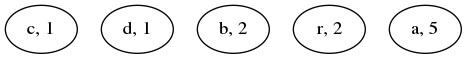
\includegraphics[scale = 0.3]{HSMI/step1.png} 
\end{center}
\'Etape 2 : Fusion des n{\oe}uds de \texttt{c} et \texttt{d} 
\begin{center}
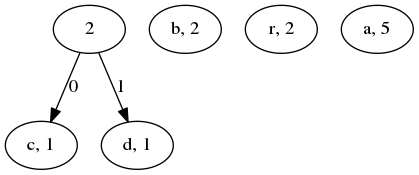
\includegraphics[scale = 0.3]{HSMI/step2.png} 
\end{center}
\'Etape 3 : Fusion des n{\oe}uds de \texttt{b} et de poids 2
\begin{center}
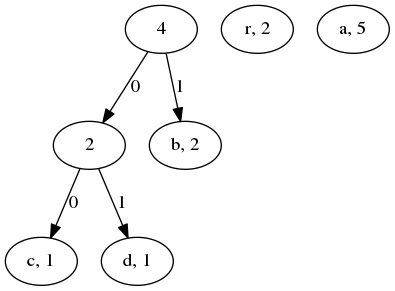
\includegraphics[scale = 0.3]{HSMI/step3.png} 
\end{center}
\'Etape 4 : Tri de la for\^et dans l'ordre croissant des poids
\begin{center}
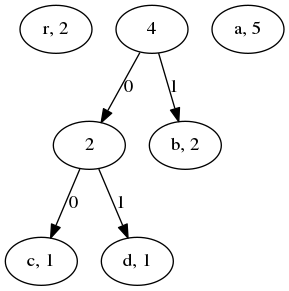
\includegraphics[scale=0.3]{HSMI/step4.png} 
\end{center}
\'Etape 5 : Fusion des n{\oe}uds de \texttt{r} et de poids 4
\begin{center}
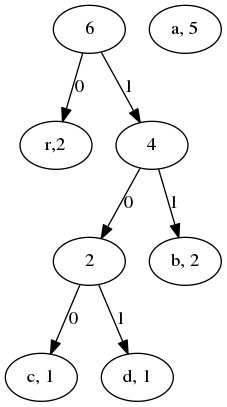
\includegraphics[scale = 0.3]{HSMI/step5.png} 
\end{center}
\'Etape 6 : Tri de la for\^et dans l'ordre croissant des poids
\begin{center}
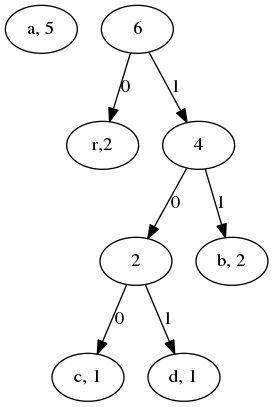
\includegraphics[scale = 0.3]{HSMI/step6.png} 
\end{center}
Ainsi, l'arbre obtenu \`a la fin est le suivant (apr\`es fusion des n{\oe}uds de \texttt{a} et de poids 6) :

\begin{figure}[H]
\begin{center}
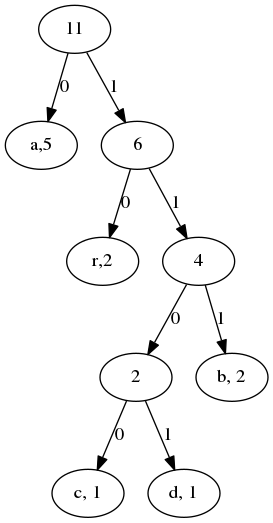
\includegraphics[scale = 0.4]{HSMI/step7.png}
\caption{Arbre de Huffman Statique pour \texttt{abracadabra}}
\end{center}
\end{figure}
L'image de abracadabra par la fonction de compression est alors : 
0\,111\,10\,0\,1100\,0\,1101\,0\,111\,10\,0 .
$\newline\newline\newline$

\subsection{Sp\'ecification}
Les fichiers compress\'es doivent avoir un format correct pour pouvoir \^etre d\'ecompresser convenablement. Dans notre algorithme, un fichier compress\'e poss\`ede un en-t\^ete qui contient 5 \'el\'ements :
\begin{enumerate}
\item Un nombre magique cod\'e sur 4 octets, qui contient exactement la cha\^ine \texttt{HSMI}
\item Un nombre cod\'e sur un octet, contenant le nombre de bits \`a lire sur le dernier octet. Ce nombre est naturellement compris entre 0 et 8.
\item Un nombre $n$ correspondant au nombre de n{\oe}ud de l'arbre, cod\'e sur 2 octets, en big endian.
\item Un nombre cod\'e sur 2 octets en big endian, correspondant \`a l'id de la racine de l'arbre.
\item On trouve enfin $n$ blocs de 7 octets. Chaque bloc contient les donn\'ees d'un n{\oe}ud de l'arbre de codage. On trouve ces 4 \'el\'ements : 
	\begin{enumerate}
		\item l'id du n{\oe}ud (compris entre 1 et $n$), cod\'e sur 2 octets en big endian.
		\item la lettre contenue dans le n{\oe}ud, cod\'e sur 1 octet.
		\item l'id du fils gauche cod\'e sur 2 octets en big endian (peut \^etre \'egal \`a 0, si le n{\oe}ud est une feuille)
		\item l'id du fils droit cod\'e sur 2 octets en big endian (peut \^etre \'egal \`a 0, si le n{\oe}ud est une feuille)
	\end{enumerate}
\end{enumerate}

\`A la suite de cet en-t\^ete, on trouve une suite finie de bits contenant les chemins permettant la d\'ecompression du fichier.
$\newline$

L'algorithme de Huffman Statique comprend deux inconv\'enients majeurs, tout d'abord, le fichier d'entr\'ee doit \^etre lu deux fois, une fois pour d\'eterminer l'arbre de codage, puis une seconde fois pour calculer l'image du texte de d\'epart, par la fonction de compression. De plus, l'arbre de compression doit \^etre transmis afin de proc\'eder \`a la d\'ecompression. L'algorithme de Huffman Dynamique permet de palier \`a ces deux inconv\'enients.


\section{Huffman Dynamique}

L'algorithme de Huffman Dynamique est, tout comme le Huffman Statique, un algorithme de compression sans perte, mais qui contrairement au premier algorithme, utilise un code \`a longueur non variable (c'est-\`a-dire que chaque symbole est cod\'e sur un nombre fix\'e de bits). 

Tout d'abord, dans ce deuxi\`eme algorithme, l'arbre de codage, est modifi\'e au cours du temps, et ne d\'epend que des symboles d\'ej\`a lus, ainsi, contrairement \`a l'algorithme pr\'ec\'edant, on peut l'appliquer sur un flux de donn\'ees continu. 

Ensuite, l'arbre de codage (qui est binaire entier), doit, \`a tout moment de l'algorithme, v\'erifier les deux propri\'et\'es suivantes : $\newline$
Soit $n+1$ le nombre de n{\oe}uds de l'arbre, $(c_i)_{i \in \llbracket 0, n \rrbracket}$ la suite de n{\oe}uds, et $p : \{c_i | i \in \llbracket 0, n \rrbracket\} \rightarrow \mathbb{N}$, qui \`a un n{\oe}ud associe son poids.
\begin{enumerate}
\item La suite $(p(c_i))_{i \in \llbracket 0, n \rrbracket}$ est croissante.
\item Pour tout $i \in \llbracket 0, \frac{n}{2} \rrbracket$, $c_{2i}$ et $c_{2i+1}$ sont fr\`eres
\end{enumerate}

Par exemple, l'arbre suivant est bien un arbre de Huffman : $\newline$

\begin{figure}[H]
	\begin{center}
		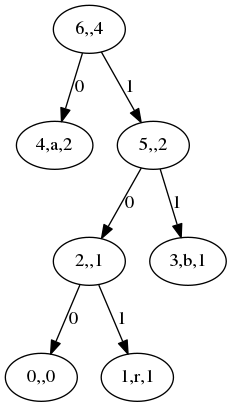
\includegraphics[scale=0.3]{HDMI/exempleArbreHuff.png}
		\caption {Exemple d'un arbre de Huffman}
	\end{center}
\end{figure}
\subsection{Fonctionnement}

\subsubsection{Manipulation de l'arbre}
Les algorithmes de compression et de d\'ecompression utilisant le m\^eme arbre, les manipulations sont les m\^emes dans les deux algorithmes. On trouve principalement 4 op\'erations sur ces arbres :

\begin{enumerate}

\item Initialisation de l'arbre
$\newline$

L'arbre est en premier lieu, initialis\'e avec un n{\oe}ud vide, d'indice 0, et de poids 0.

\item Ajout d'un nouveau symbole 
$\newline$

Soit $A$ l'arbre courant. $\newline$
Lors de la lecture d'un caract\`ere $k$, s'il n'a jamais \'et\'e rencontr\'e auparavant, on l'ajoute dans l'arbre de la mani\`ere suivante : $\newline$
Soit $d_0$ un nouveau n{\oe}ud, qui est une feuille, de poids 0, et de caract\`ere vide. $\newline$
Soit $d_1$ un nouveau n{\oe}ud, qui est une feuille, de poids 1, et de caract\`ere $k$. $\newline$
Soit $d_2$ un nouveau n{\oe}ud, de poids 0, et de caract\`ere vide, qui a pour fils gauche le n{\oe}ud $d_0$ et pour fils droit le n{\oe}ud $d_1$. $\newline$
On remplace alors le n{\oe}ud $c_0$ par le noeud $d_2$ dans l'arbre $A$.
La suite $(c_i)_{i \in \llbracket 0, n \rrbracket}$ est alors actualis\'ee (on augmente l'indice de tout les n{\oe}uds de 2).
On proc\`ede ensuite \`a un r\'e\'equilibrage \`a partir du n{\oe}ud $d_2$. $\newline$
L'illustration suivante est un exemple d'ajout :
\begin{figure}[H]
	\begin{center}
	\includegraphics[scale=0.3]{HDMI/AjoutAbrac.png}
	\caption{Ajout du caract\`ere c dans l'arbre de gauche}
	\end{center}
\end{figure}

\item Cas d'un caract\`ere d\'ej\`a lu
$\newline$

Si le caract\`ere lu est d\'ej\`a apparu dans le texte auparavant, alors il se trouve dans l'arbre, on lance alors une proc\'edure de r\'e\'equilibrage \`a partir de son n{\oe}ud.

\item R\'e\'equilibrage 
$\newline$

Un r\'e\'equilibrage sert \`a conserver la premi\`ere propri\'et\'e des arbres de Huffman.
On effectue un r\'e\'equilibre uniquement apr\`es avoir ajout\'e un caract\`ere, ou lorsque l'on veut incr\'ementer le poids d'un n{\oe}ud.
Pour cela, on effectue la proc\'edure suivante : $\newline$
Soit $c_i$ le n{\oe}ud depuis lequel on commence le r\'e\'equilibrage. $\newline$
Tant que $c_i$ n'est pas la racine de l'arbre : $\newline$
On cherche si il existe un $j \geqslant i$, le plus grand possible, tel que le $p(c_i) \leqslant p(c_j)$, et tel que $c_j$ n'est pas le p\`ere de $c_i$. $\newline$
Si un tel $j$ existe, on \'echange les valeurs de $c_j$ et de $c_i$. $\newline$
On incr\'emente alors la valeur du poids de $c_i$. $\newline$
Puis on passe au p\`ere de $c_i$. $\newline$
L'exemple suivant montre un r\'e\'equilibrage :
\begin{figure}[H]
	\begin{center}
		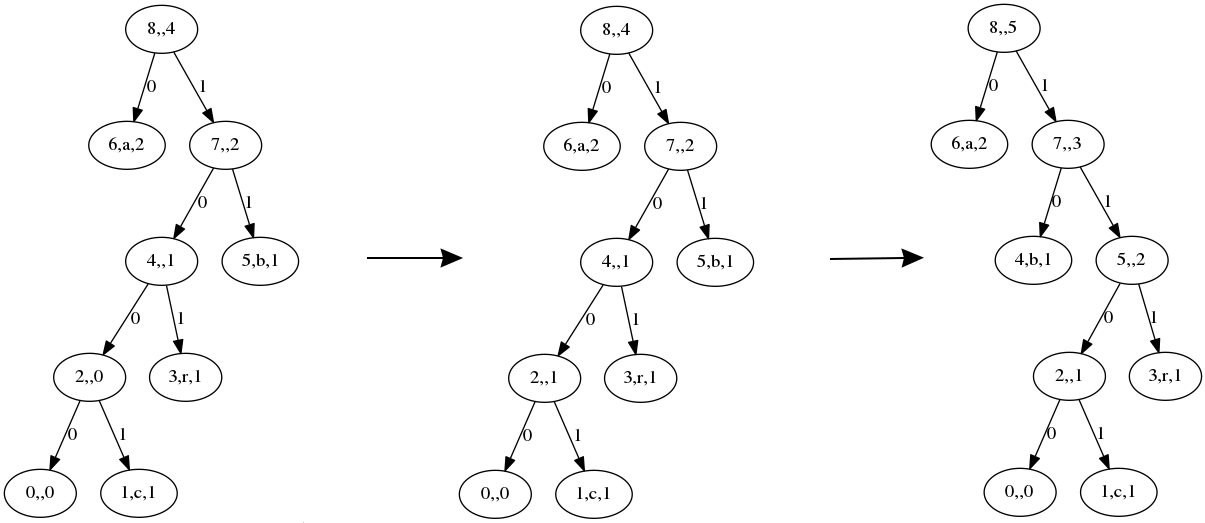
\includegraphics[scale=0.3]{HDMI/ReeqC.png}
		\caption {Exemple de r\'e\'equilibrage apr\`es ajout de c}
	\end{center}
\end{figure}

\end{enumerate}

\subsubsection{Compression}

\`A chaque lecture de caract\`ere, si le caract\`ere est un nouveau symbole, on \'ecrit le chemin de la racine, au n{\oe}ud $c_0$, puis on \'ecrit le caract\`ere lu.
Si le caract\`ere a d\'ej\`a \'et\'e rencontr\'e auparavant, on \'ecrit le chemin de la racine au n{\oe}ud du caract\`ere.

\subsubsection{D\'ecompression}

La d\'ecompression se d\'eroule de la mani\`ere suivante :

On se place \`a la racine de l'arbre.

Tant qu'on a des bits \`a lire :

On lit un bit, si il vaut 1, on descend dans le fils gauche, sinon on descend dans le fils droit.

Si on n'est pas dans une feuille, on continue la lecture et l'avanc\'ee dans le parcours de l'arbre.
Sinon, on est dans une feuille, et alors :

Si on est dans la feuille vide (on est dans $c_0$), on lit un caract\`ere, pour obtenir le caract\`ere cod\'e, et on le rajoute \`a l'arbre, puis on proc\`ede \`a un r\'e\'equilibrage, par rapport au n{\oe}ud $c_2$ (le nouveau p\`ere du n{\oe}ud $c_0$).

Sinon, on est dans une feuille qui contient un caract\`ere, on lance un r\'e\'equilibrage sur cette feuille, et on \'ecrit le caract\`ere.


\subsection{Structures de donn\'ees utilis\'ees}

L'algorithme de Huffman Dynamique utilisant principalement un arbre binaire, une structure d'arbre binaire a naturellement \'et\'e choisie. De plus, l'arbre binaire est rang\'e dans un tableau, car l'acc\`es \`a chaque n{\oe}ud est facilit\'e. Chaque n{\oe}ud contient un caract\`ere si c'est une feuille, les distances entre l'indice du n{\oe}ud courant, et l'indice du fils gauche, du fils droit, et du p\`ere, un poids (qui correspond au nombre de caract\`ere du n{\oe}ud d\'ej\`a lu). Le rangement dans un tableau facilite aussi la gestion des indices pour chaque n{\oe}ud, et la recherche d'un noeud de poids \'egale, d'indice plus grand. Garder la distance nous permet d'\'eviter de mettre \`a jour les pointeurs vers les fils gauches, et droits, des n{\oe}uds fils d'un n{\oe}ud qui a \'et\'e \'echang\'e avec un autre durant un r\'e\'equilibrage.
 
Une deuxi\`eme structure de donn\'ees utilis\'ee est un tableau d'indice inverse, de taille 256 (une case pour chaque valeur ASCII possible), qui a un caract\`ere, associe deux attributs :
\begin{enumerate}
\item l'indice du n{\oe}ud de l'arbre, qui contient le caract\`ere, utilis\'e pour acc\'eder au n{\oe}ud en temps constant, et pour savoir si le caract\`ere est un nouveau caract\`ere ou non. 
\item le chemin de la racine, au n{\oe}ud pr\'ec\'edemment cit\'e.
On conserve un tel chemin, afin d'\'eviter de le recalculer \`a chaque fois qu'on rencontre un caract\`ere.
\end{enumerate}

\subsection{Optimisation}

Dans une premi\`ere impl\'ementation de l'algorithme, un tableau contenant les caract\`eres d\'ej\`a rencontr\'es \'etait maintenu \`a jour. Cependant, pour pouvoir utiliser ce tableau pour un caract\`ere $c$, il fallait effectuer une recherche lin\'eaire, donc en $\theta($Nombre de caract\`eres diff\'erents$)$.
De plus, si on a d\'ej\`a rencontr\'e le caract\`ere auparavant, on doit \'ecrire le chemin de la racine, au n{\oe}ud contenant ce caract\`ere, et lancer un r\'e\'equilibre, ce qui demande alors de parcourir l'arbre, jusqu'\`a trouver le bon n{\oe}ud, et donc une seconde recherche dans l'arbre, en $\theta($Nombre de n{\oe}ud de l'arbre$)$.

Une optimisation possible est de cr\'eer un tableau associatif, de 256 cases (le nombre de caract\`eres ASCII possibles), qui a un char $c$, associe une valeur particuli\`ere, si $c$ n'a jamais \'et\'e vu, ou un pointeur sur le n{\oe}ud et le chemin demand\'e sinon, on \'economise alors les deux recherches, passant alors d'un $\theta($Nombre de n{\oe}ud de l'arbre + Nombre de caract\`eres diff\'erents$)$ \`a un $\theta(1)$. Ce tableau est alors mis \`a jour \`a chaque r\'e\'equilibrage, en cas de besoin.

De plus, la recherche d'un p\`ere de poids \'egale au poids du n{\oe}ud courant (qui est la recherche la plus effectu\'ee) s'effectuait en temps lin\'eaire avant, pour ensuite passer \`a une recherche dichotomique (Les poids \'etant tri\'es dans l'ordre croissant).
\newpage
\subsection{Exemple}


Les \'etapes du codage de \texttt{abracadabra} sont les suivantes :

\begin{longtable}{| c | c | c | c |}
\hline
\'Etape & Code g\'en\'er\'e & Arbre & Description \\
\hline
\raisebox{1ex}{1} &  & 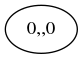
\includegraphics[scale = 0.3]{HDMI/exinit.png} 
& \raisebox{1ex}{Initialisation}\\ \hline
\raisebox{5ex}{2} & \raisebox{5ex}{a} & 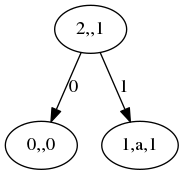
\includegraphics[scale = 0.3]{HDMI/ex01.png} 
& \raisebox{5ex}{Ajout de \texttt{a}}\\ \hline
\raisebox{9.5ex}{3} & \raisebox{9.5ex}{0b} & 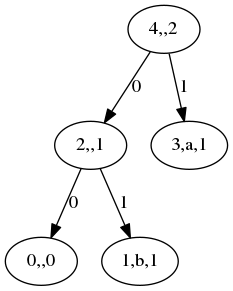
\includegraphics[scale = 0.3]{HDMI/ex02.png} 
& \raisebox{9.5ex}{Ajout de \texttt{b}}\\ \hline
\raisebox{14ex}{4} & \raisebox{14ex}{00r} & 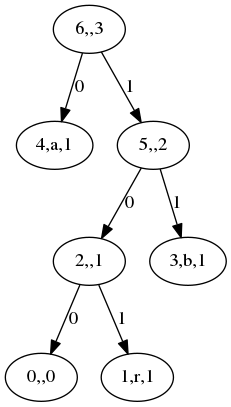
\includegraphics[scale = 0.3]{HDMI/ex03.png} 
& \raisebox{14ex}{Ajout de \texttt{r}}\\ \hline
\raisebox{12.5ex}{5} & \raisebox{12.5ex}{0} & 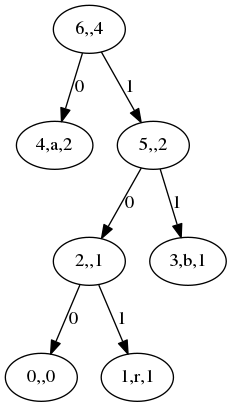
\includegraphics[scale = 0.3]{HDMI/ex04.png} 
& \raisebox{12.5ex}{Incr\'ementation de \texttt{a}}\\ \hline
\raisebox{17.5ex}{6} & \raisebox{17.5ex}{100c} & 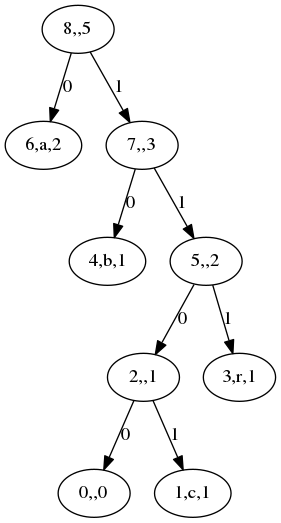
\includegraphics[scale = 0.3]{HDMI/ex05.png} 
& \raisebox{17.5ex}{Ajout de \texttt{c}} \\ \hline
\raisebox{17.5ex}{7} & \raisebox{17.5ex}{0} & 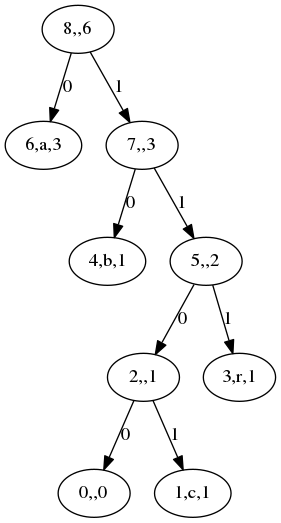
\includegraphics[scale = 0.3]{HDMI/ex06.png} 
& \raisebox{17.5ex}{Incr\'ementation de \texttt{a}}\\ \hline
\raisebox{16ex}{8} & \raisebox{16ex}{1100d} & 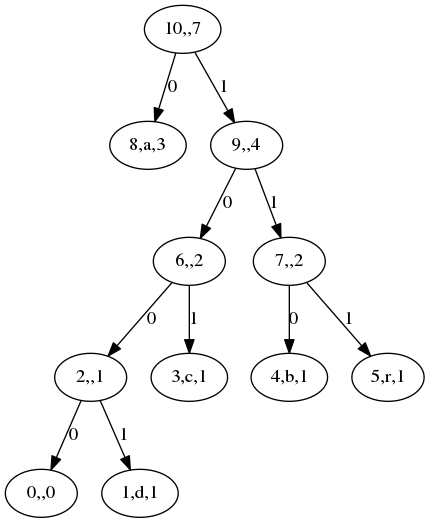
\includegraphics[scale = 0.3]{HDMI/ex07.png} 
& \raisebox{16ex}{Ajout de \texttt{d}}\\ \hline
\raisebox{17.5ex}{9} & \raisebox{17.5ex}{0} & 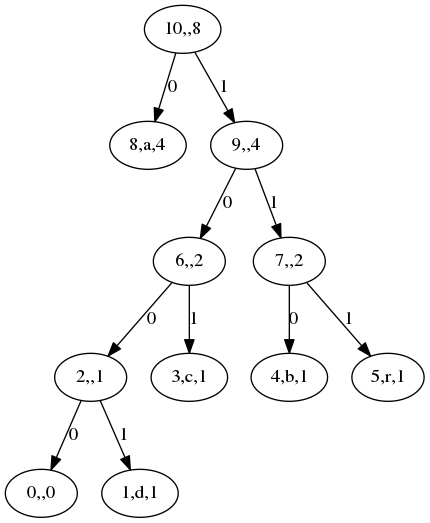
\includegraphics[scale = 0.3]{HDMI/ex08.png} 
& \raisebox{17.5ex}{Incr\'ementation de \texttt{a}}\\ \hline
\raisebox{17.5ex}{10} & \raisebox{17.5ex}{111} & 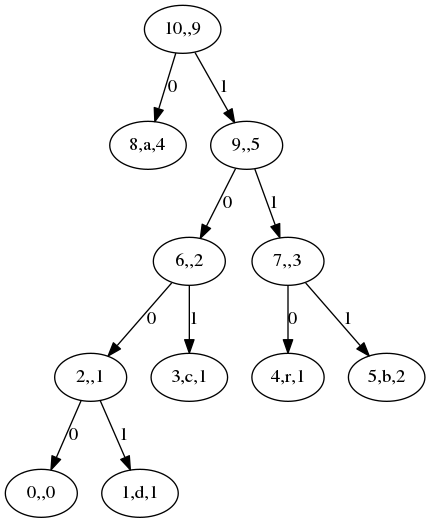
\includegraphics[scale = 0.3]{HDMI/ex09.png} 
& \raisebox{17.5ex}{Incr\'ementation de \texttt{b}}\\ \hline
\raisebox{17.5ex}{11} & \raisebox{17.5ex}{110} & 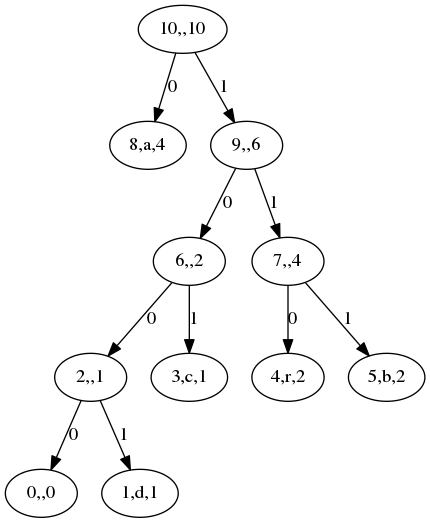
\includegraphics[scale = 0.3]{HDMI/ex10.png} 
& \raisebox{17.5ex}{Incr\'ementation de \texttt{r}}\\ \hline
\raisebox{17.5ex}{12} & \raisebox{17.5ex}{0} & 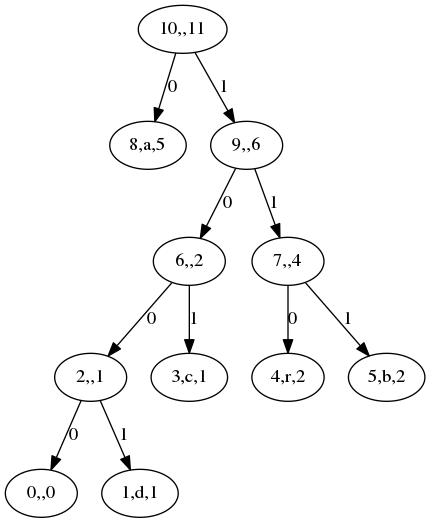
\includegraphics[scale = 0.3]{HDMI/ex11.png} 
& \raisebox{17.5ex}{Incr\'ementation de \texttt{a}}\\
\hline


\end{longtable}

\subsection{Sp\'ecification}
Tout comme pour l'algorithme pr\'ec\'edant, les fichiers compress\'es doivent respecter un certain format pour pouvoir \^etre d\'ecompress\'e.
Pour cet algorithme, chaque fichier poss\`ede un en-t\^ete, contenant la cha\^ine \texttt{HDMI} cod\'e sur 4 octets.
\`A la suite de cet en-t\^ete, on trouve une suite finis de bits, correspondant au codage du fichier original.

L'algorithme devant fonctionner sur un flux de donn\'ees, la cr\'eation d'un caract\`ere de fin de fichier est n\'ecessaire. Cependant, un fichier quelconque peut contenir tout les caract\`eres codables sur 8 bits (soit 1 octet). C'est pour cela qu'au lieu de coder nos caract\`eres sur 1 octet, on le code sur 2. Le premier octet vaut \texttt{11111111} si le caract\`ere correspond au caract\`ere de fin de fichier, et \texttt{00000000} sinon.
De plus, pour savoir qu'il faut lire un caract\`ere (donc 2 octets) lors de la d\'ecompression, on a besoin du chemin de la racine, au n{\oe}ud de poids 0. C'est pour cela qu'une fois que la compression du fichier d'origine est termin\'ee, on \'ecrit le chemin de la racine de l'arbre de codage, au n{\oe}ud de poids 0, puis le caract\`ere \texttt{11111111\,00000000}.


\section{Pseudo-code}

\subsection{Huffman Statique Compression}

\begin{algorithm}[H]
\caption{Compression Huffman Statique Construction de l'arbre}
\begin{algorithmic} 
\REQUIRE $\newline$
$T$ : le texte \`a compresser$\newline$
$F$ : le ableau des fr{\'e}quences (vide) $\newline$
\WHILE {$X \neq EOF$}
\STATE $X \leftarrow litUnCaractere(T)$
\IF {$F$ contient $X$}
\STATE $F[X].p \leftarrow F[X].p + 1$	
\ELSE 
\STATE $F \leftarrow F \cup \{(X, 1)\}$
\ENDIF
\ENDWHILE

\WHILE {longueur de $F \neq 1$}
\STATE $F \leftarrow tri(F)$
\STATE $n \leftarrow nouveau Noeud$
\STATE $n.p \leftarrow F[0].p + F[1].p$
\STATE $n.fg \leftarrow F[0]$
\STATE $n.fd \leftarrow F[1]$
\STATE $F \leftarrow (F \backslash \{F[0], F[1]\}) \cup \{n\}$
\ENDWHILE

\end{algorithmic}
\end{algorithm}

\begin{algorithm}[H]
\caption{Compression Huffman Statique Codage du texte}
\begin{algorithmic} 
\REQUIRE $\newline$
$T$ : le texte \`a compresser $\newline$
$F$ : l'arbre de codage$\newline$
\WHILE {$X \neq EOF$}
\STATE $X \leftarrow litUnCaractere(T)$
\STATE $C \leftarrow codeDe(X)$ dans $F$
\STATE \'Ecrit $C$
\ENDWHILE
\end{algorithmic}
\end{algorithm}

\subsection{Huffman Statique D\'ecompression}
\begin{algorithm}[H]
\caption {D\'ecompression Huffman Statique}
\begin{algorithmic}
\REQUIRE $\newline$
$F$ Arbre des fr\'equences $\newline$
$T$ suite finie de bits $\newline$
$N \leftarrow F.root\newline$
\WHILE {Il reste des bits \`a lire}
\STATE $X \leftarrow litUnBit(T)$
\IF {$X = 0$}
\STATE $N \leftarrow N.fg$
\ELSE
\STATE $N \leftarrow N.fd$ 
\ENDIF
\IF {$N$ est une feuille}
\STATE \'Ecrit $N.c$
\STATE $N \leftarrow F.root$
\ENDIF
\ENDWHILE
\end{algorithmic}
\end{algorithm}


\subsection{Huffman Dynamique Compression}

\begin{algorithm}[H]
\caption{Compression Huffman Dynamique}
\begin{algorithmic}
\STATE //la fonction reequilibre renvois \`a la fonction d\'efinie en dessous
\REQUIRE $\newline$
$T$ texte \`a compresser $\newline$
$A \leftarrow initArbre()$

\WHILE {$X \neq EOF$}
\STATE $X \leftarrow litUnCaractere(T)$
\IF {$dejaVu(A, X)$} 
\STATE $Nx \leftarrow getNoeud(A, X)$
\STATE $EcritLeCheminDeLaRacineA(Nx)$
\STATE $reequilibre(Nx, A)$
\ELSE 
\STATE $c_0 \leftarrow getNoeudDePoids0(A)$
\STATE $EcritLeCheminDeLaRacineA(c_0)$
\STATE $Ecrit(X)$
\STATE $ajouteDans(A, X)$ //Peut \^etre vide, ajouteDans rajoute le caract\`ere X dans l'arbre, et renvois le p\`ere du n{\oe}ud de poids 0
\STATE $reequilibre(c_0, A)$ //$c_0$ qui \'etait l'ancien n{\oe}ud de poids 0, est maintenant son p\`ere apr\`es l'ajout du caract\`ere X
\ENDIF
\ENDWHILE
\end{algorithmic}
\end{algorithm}

\begin{algorithm} [H]
\caption {Algorithme de r\'e\'equilibrage de l'arbre}
\begin{algorithmic}
\REQUIRE $\newline$
$n$ n{\oe}ud de d\'epart pour le r\'e\'equilibrage $\newline$
$A$ arbre

\WHILE {$n \neq root(A)$}
\IF {Il y a un n{\oe}ud $c_k$ d'indice plus haut que n \&\& de poids \'egal \&\& qui n'est pas son p\`ere}
\STATE $echange(X, c_k)$
\STATE $incrementPoids(n)$
\STATE $n \leftarrow Pere(n)$
\ENDIF
\ENDWHILE
\STATE $incrementPoids(n)$
\end{algorithmic}
\end{algorithm}

\subsection{Huffman Dynamique D\'ecompression}

\begin{algorithm}[H]
\caption{D\'ecompression Huffman Dynamique}
\begin{algorithmic}
\REQUIRE $\newline$
$T$ texte \`a d\'ecompresser $\newline$
$A \leftarrow initArbre()$ $\newline$
$N \leftarrow racine(A)$ $\newline$

\WHILE{Il reste des bits \`a lire}
\STATE $X \leftarrow litUnBit(T)$
\IF {$X = 0$}
\STATE $N \leftarrow N.fg$
\ELSE
\STATE $N \leftarrow N.fd$
\ENDIF
\IF {$isLeaf(N)$}
\IF {$N.c = \emptyset$}
\STATE $c \leftarrow litUnCaractere(T)$
\STATE $ajouteDans(A, c)$
\STATE $ecrit(c)$
\ELSE 
\STATE $ecrit(N.c)$
\ENDIF
\STATE $reequilibre(N, A)$
\STATE $N \leftarrow racine(A)$
\ENDIF
\ENDWHILE
\end{algorithmic}
\end{algorithm}

\newpage
\section{Performances}
Pour l'ensemble des graphiques suivants, \texttt{HSMI} d\'esigne l'algorithme Huffman Statique, \texttt{HDMI Non opti} d\'esigne l'algorithme Huffman Dynamique sans optimisation, et enfin, \texttt{HDMI Opti} renvoie \`a l'algorithme Huffman Dynamique, apr\`es optimisation.

\subsection{Fichiers texte}
\begin{center}
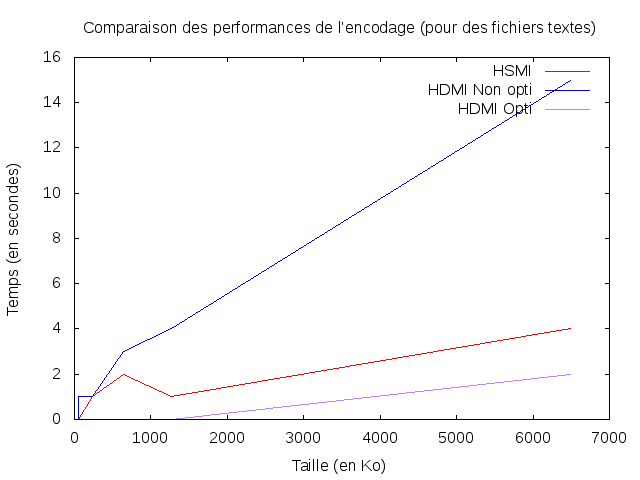
\includegraphics[scale=0.5]{Perf/txt/encodecomptxt2.png}
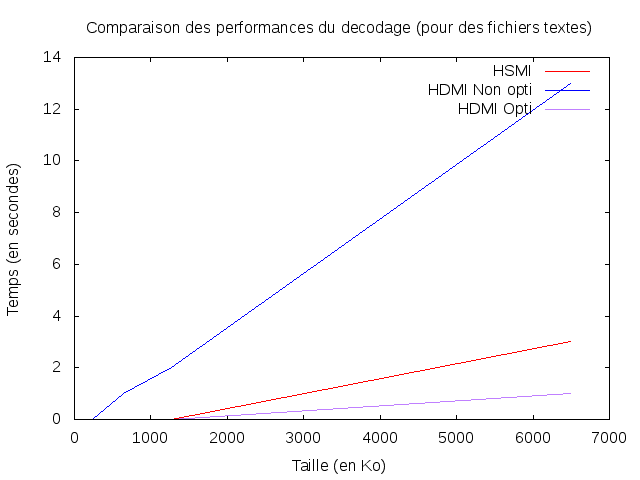
\includegraphics[scale=0.5]{Perf/txt/decodecomptxt2.png}
\end{center}

\subsection{Fichiers image}
\begin{center}
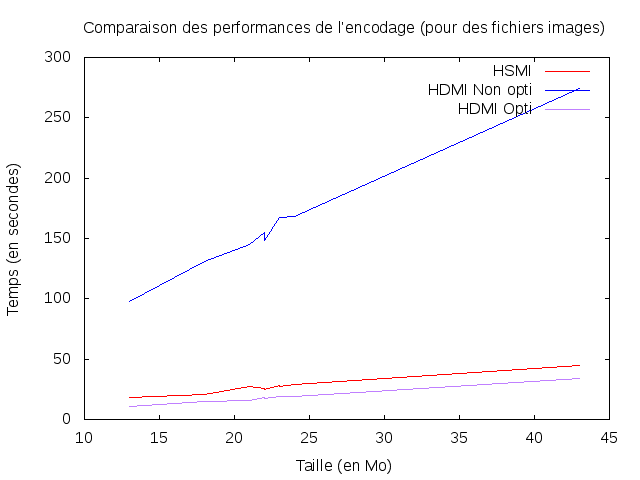
\includegraphics[scale=0.5]{Perf/img/encodecompimg2.png}
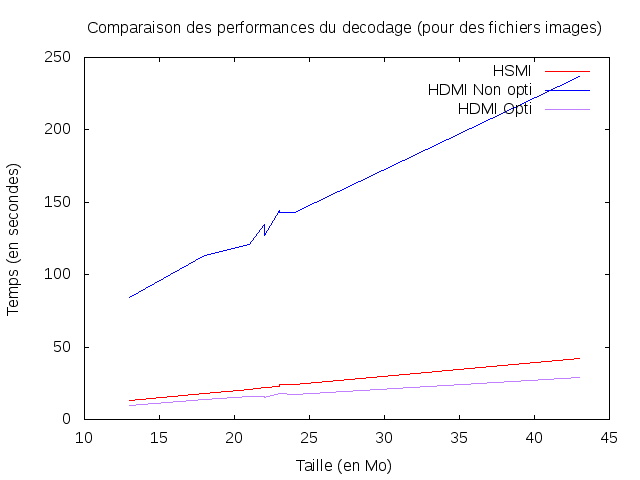
\includegraphics[scale=0.5]{Perf/img/decodecompimg2.png}
\end{center}

\subsection{Fichiers audio}
\begin{center}
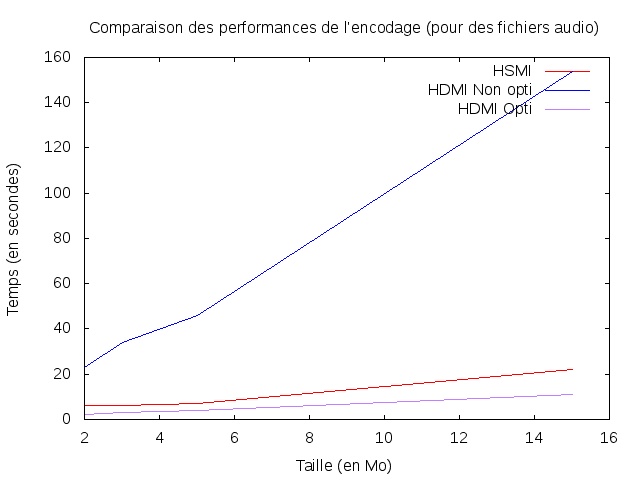
\includegraphics[scale=0.5]{Perf/audio/encodecompaudio2.png}
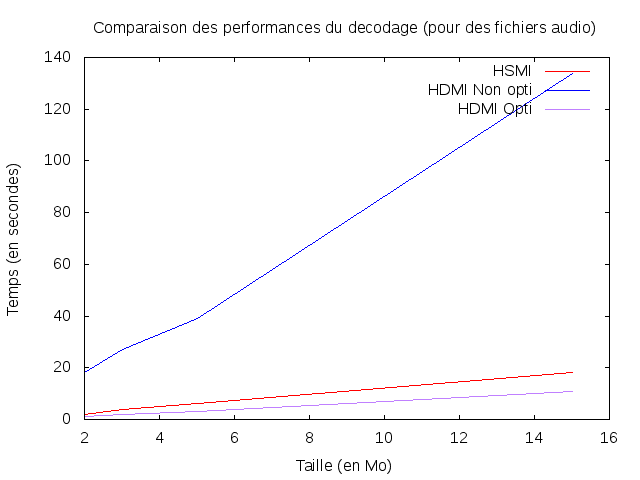
\includegraphics[scale=0.5]{Perf/audio/decodecompaudio2.png}
\end{center}

\subsection{Comparaison des taux de compression}

\begin{center}
\begin{tabular}{|l|c|r|}
  \hline
  Nom du fichier & Type du fichier & Taille du fichier (Ko) \\
  \hline
  $i_1 : pinngd\_mlc$ & nef & 13956 \\
  $i_2 : rnmyic$ & dng & 18514 \\
  $i_3 : uzkoci\_razberry$ & nef & 21236 \\
  $i_4 : juriart$ & cr2 & 22512  \\
  $i_5 : stsci$ & tif & 22612 \\
  $i_6 : emdde7$ & raf & 23305 \\
  $i_7 : elbebe1991$ & cr2 & 23811 \\
  $i_8 : mr.wolf$ & dng & 24810 \\
  $i_9 : stci2$ & tif & 43460 \\
  \hline
  $a_1 : muscle$ & wav & 2228 \\
  $a_2 : airplane$ & wav & 2494 \\
  $a_3 : swimming$ & wav & 3700 \\
  $a_4 : car$ & wav & 5594 \\
  $a_5 : rain$ & wav & 15245 \\
  \hline
  $t_1 : amerikasta$ & txt & 46 \\
  $t_2 : ourfriendthedog$ & txt & 49\\
  $t_3 : florante$ & txt & 237 \\
  $t_4 : chinois$ & txt & 641 \\
  $t_5 : mobydick$ & txt & 1270 \\
  $t_6 : sherlock$ & txt & 6488 \\
  \hline
\end{tabular}


$\newline$
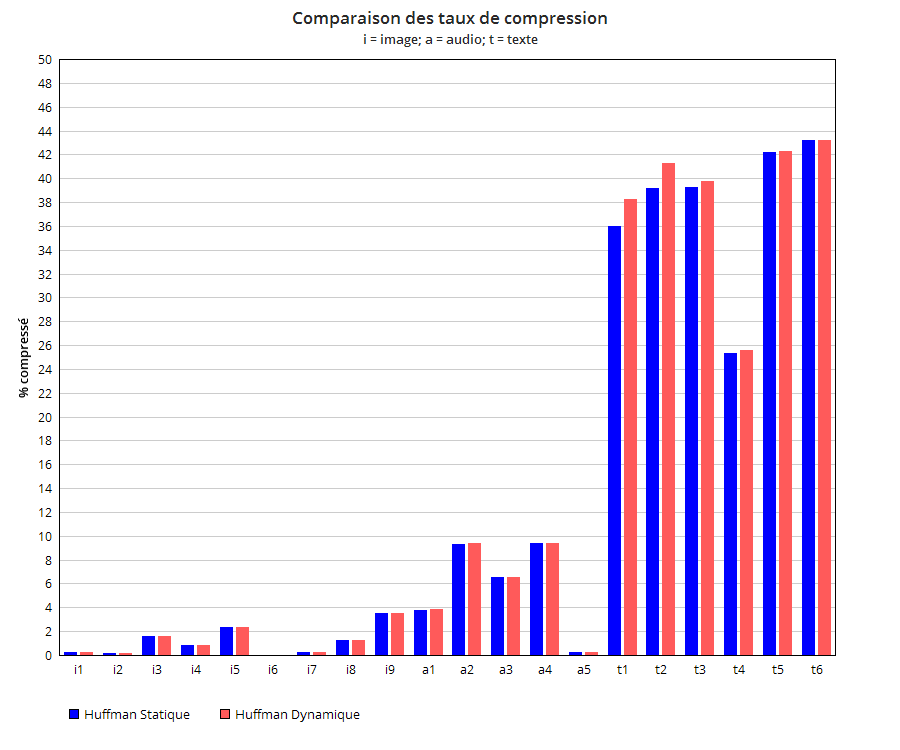
\includegraphics[scale=0.35]{Perf/compTxCompress.png}
\end{center}
Sur ce graphique, on voit que les algorithmes sont tr\`es peu efficace pour les fichier image et audio, car les images prises en test ont toutes des formats de fichier compress\'es.
Enfin, on voit que la compression sur des fichiers textes est d'environ 40\% sauf pour le 4\`eme fichier. Cette diff\'erence s'explique par le fait que ce fichier est un texte en chinois, cod\'e en UTF-8. Or l'UTF-8 utilise un code \`a longueur variable pour encoder les caract\`eres. De plus, les symboles encodables sur 1 octet en UTF-8 correspondent exactement \`a ceux de la table ASCII. Donc tout les caract\`eres usuels sont cod\'es sur 1 octet, contrairement aux caract\`eres chinois, qui sont cod\'es sur plusieurs octets. Une solution pour obtenir un bon taux de compression serait de lire le bon nombre d'octet \`a chaque lecture de caract\`ere.



\section{Liste des outils utilis\'es}

\noindent Les graphes d'arbres ont \'et\'e g\'en\'er\'es \`a l'aide du logiciel \href{http://www.graphviz.org/}{GraphViz}. $\newline$
Les diff\'erents graphiques ont \'et\'e con{\c c}us gr\^ace \`a l'outil \href{http://www.gnuplot.info/}{gnuplot}
\newpage
\section*{Conclusion}

Comme nous avons pu le constater, les deux versions de l'algorithme de Huffman sont \'equivalentes dans leurs versions optimis\'ees, aussi bien en temps qu'en taux compression. Les algorithmes fonctionnent en temps lin\'eaire et la complexit\'e ne change pas ou peu en fonction du type de fichier. 
\newline N\'eanmoins, les taux de compressions ne sont correctes que pour des fichiers textes qui sont de l'ordre de 40\% ce qui s'explique par le fait que les fichiers audio et image soient compress\'es. Ces algorithmes ne sont donc que tr\`es peu efficaces sur des fichiers quelconque, et ne sont pas adapt\'es \`a une utilisation \`a grande \'echelle.

\section* {Bibliographie}

L'ensemble des fichiers textes ont \'et\'e pris sur le site : \url{http://www.gutenberg.org/}.

Les fichiers audio proviennent de : \url{http://soundbible.com/tags-raw.html}

Les images utilis\'es pour les tests proviennent de :
\begin{enumerate}
\item \url{ https://www.wesaturate.com/}
\item \url{http://hubblesite.org/get_involved/hubble_image_processors/}
\end{enumerate}

\url{http://www2.ift.ulaval.ca/~dadub100/cours/H16/4003/02Acetates2.pdf}

\url{http://utbm2004.free.fr/LO42/codage\%20de\%20huffman\%20-\%20\%E9nonc\%E9.pdf}

\url{https://en.wikipedia.org/wiki/Huffman_coding}

C.Choffrut, Universi\'e Paris 7, Codage de Huffman
\end{document}

